\chapter{Introduction}\label{sec:intro}
Theoretically, fuel efficiency increases concomitantly with increasing turbine inlet temperature, but the lack of suitable materials with higher temperature capabilities (Figure~\ref{fig:TET}) has resulted in diminishing returns in fuel burn over the last 30 years (Figure~\ref{fig:FuelBurn}).  Additionally, Dimiduk and Perepezko have recently shown that, on the contrary, over the last 70 years, marginal jet engine fuel efficiency has in fact decreased with rising turbine inlet temperatures ~\cite{dimiduk03} due to the energy required to operate the intricate cooling systems required by the 2$^{nd}$ and 3$^{rd}$ generation nickel-base superalloys used in the hot sections of commercial jet engines.  Using alternative materials that do not require cooling at current operating temperatures will result in improvements in engine efficiency.
%
\begin{figure}[htbp]
\begin{center}
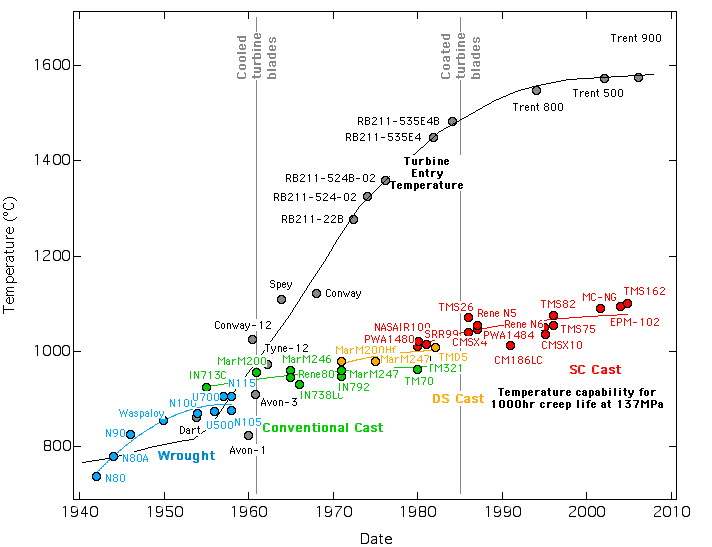
\includegraphics[width=\textwidth]{TET}
\caption{Evolution of the turbine entry temperature (TET) capability of Roll-Royce's civil aeroengines, from 1940 to present.}\label{fig:TET}
\end{center}
\end{figure}
%
\begin{figure}[htbp]
\begin{center}
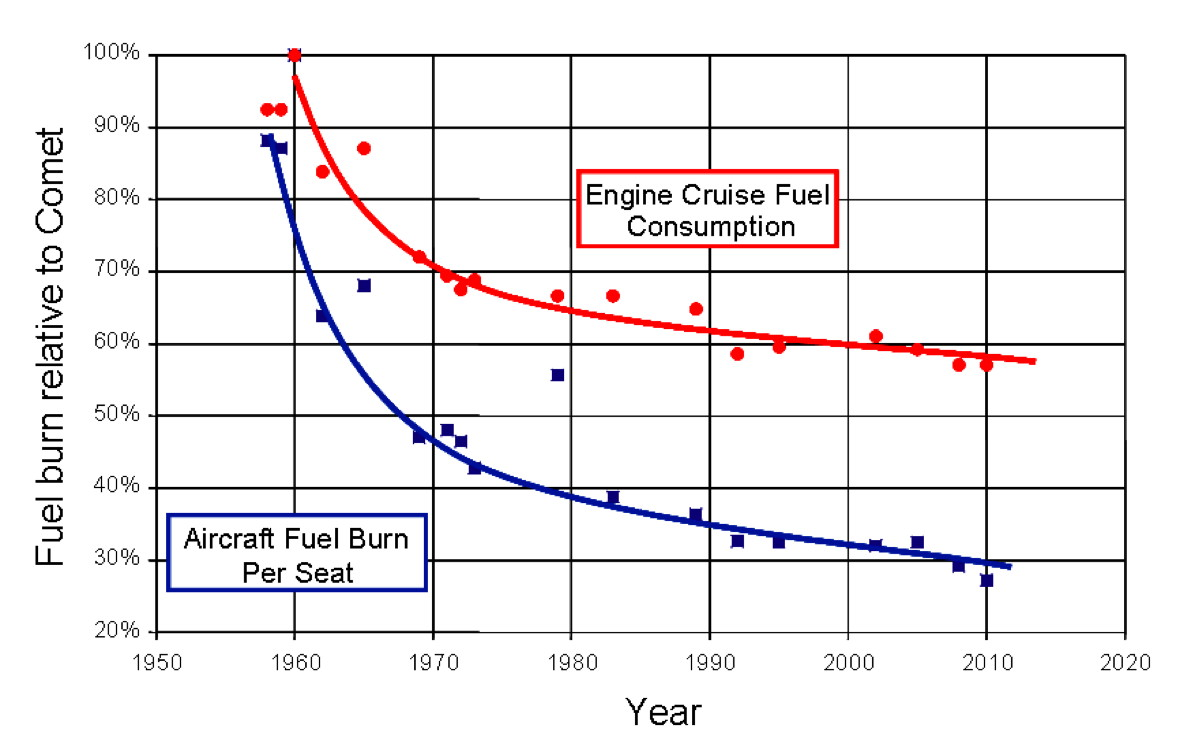
\includegraphics{FuelBurn}
\caption{Fuel burn of Rolls-Royce's civil jet engines, relative to the Comet, from 1960 to present. (Data courtesy of Rolls-Royce masterclass)}\label{fig:FuelBurn}
\end{center}
\end{figure}
%

We want to understand the issues to be faced when designing materials to supersede the commercial nickel-base superalloys used currently.  Superalloys have enjoyed unparalleled success for the last 80 years as the high temperature load-bearing material to use ~\cite{reed06}, and there are solid reasons for this.  They have high homologous temperatures, are very resistant to mechanical degradation at high operating temperatures, possess excellent environmental resistance, and are robust, tough and easily machinable ~\cite{betteridge87, sims87}. Knowing how superalloys have evolved, and understanding the difficulties encountered and the successes celebrated thus far by the nickel-base superalloy community provides the starting point for this thesis.  An investigation of the most advanced 4$^{th}$ generation superalloys forms the first part of this thesis; the second part is an examination of potential replacement systems and some preliminary results from these materials. 

The incremental approach taken has been to design superalloys with higher temperature capabilities ~\cite{reed06, cumpsty97}.  There have been three recognised generations of superalloys defined by alloy composition range.  The latest 4$^{th}$ generation superalloys are distinguished by the presences of ruthenium.  Ruthenium was found to suppress topologically close-packed (TCP) phase precipitatation very effectively with little observable detriment to the other desirable properties of superalloys ~\cite{yeh04}.  This permitted the concentration of rhenium, a powerful solid-solution strengthener, to be almost doubled without substantial reductions in microstructural stability.  These advanced superalloys with high refractory contents have more highly negative lattice misfits than earlier superalloys, and would directionally coarsen more easily upon the presence of applied stress.  These coarsened precipitates, also known as rafts, are beneficial against high temperature creep.  However, it turns out that such early-stage rafting invariably compromises intermediate temperature creep properties, allowing dislocations to cut through $\gamma$' rafts more easily than through unrafted, finer, cubiodal precipitates ~\cite{hobbs08}.  Understanding the factors that induce early-stage rafting would enable us to determine how to effectively manage them. 

More radical alternative materials to superalloys include two broad classes of materials: intermetallics and ceramics.  They offer substantial increases in temperature capability, but have many problems that have not been surmounted as of yet ~\cite{chang91, fleischer94, fleischer85a,  jackson96, kelly91, kelly96, kumar94,miracle94b, sauthoff88, shah92}.  Most notably, their inherent low ductilities and fracture-toughnesses at room temperature cause them to have low impact tolerances and to be extremely difficult to process and machine.  In this work, compositions that have the potential to offer a 100\celsius\ increase in temperature capability over current commercial superalloys will be listed.  Systems of compositions that have the potential to realise room temperature fracture-toughness and ductility that are higher than current candidate intermetallics and ceramics, while providing the desired increase in temperature capability, will be identified.  From literature, eutectic systems with a solid-solution toughening phase and a silicide load-bearing phase demonstrate the capacity to fulfill the stated aims.  These (Cr,V)$_{solid\ solution}$--(Cr,V)$_3$Si$_{intermetallic}$ eutectics will be characterised to understand their microstructural stability, failure mechanisms, high temperature creep mechanisms and oxidation character.
 
\chapter{Nickel-Base Superalloys}
\section{The Evolution of Nickel-Base Superalloys}

Sims' introduction of the origins of superalloy development in \emph{Superalloys II} ~\cite{sims87} and \emph{The Superalloys} by Reed ~\cite{reed06} both provide excellent overviews on this subject and should be consulted for more detail.  Figure~\ref{fig:evolution} beautifully sums up the evolution of nickel-base superalloys from conception in the 1930s to date, with strengthening phases shown in the top half, and the deleterious phases in the bottom half.
%
\begin{figure}[htbp]
\begin{center}
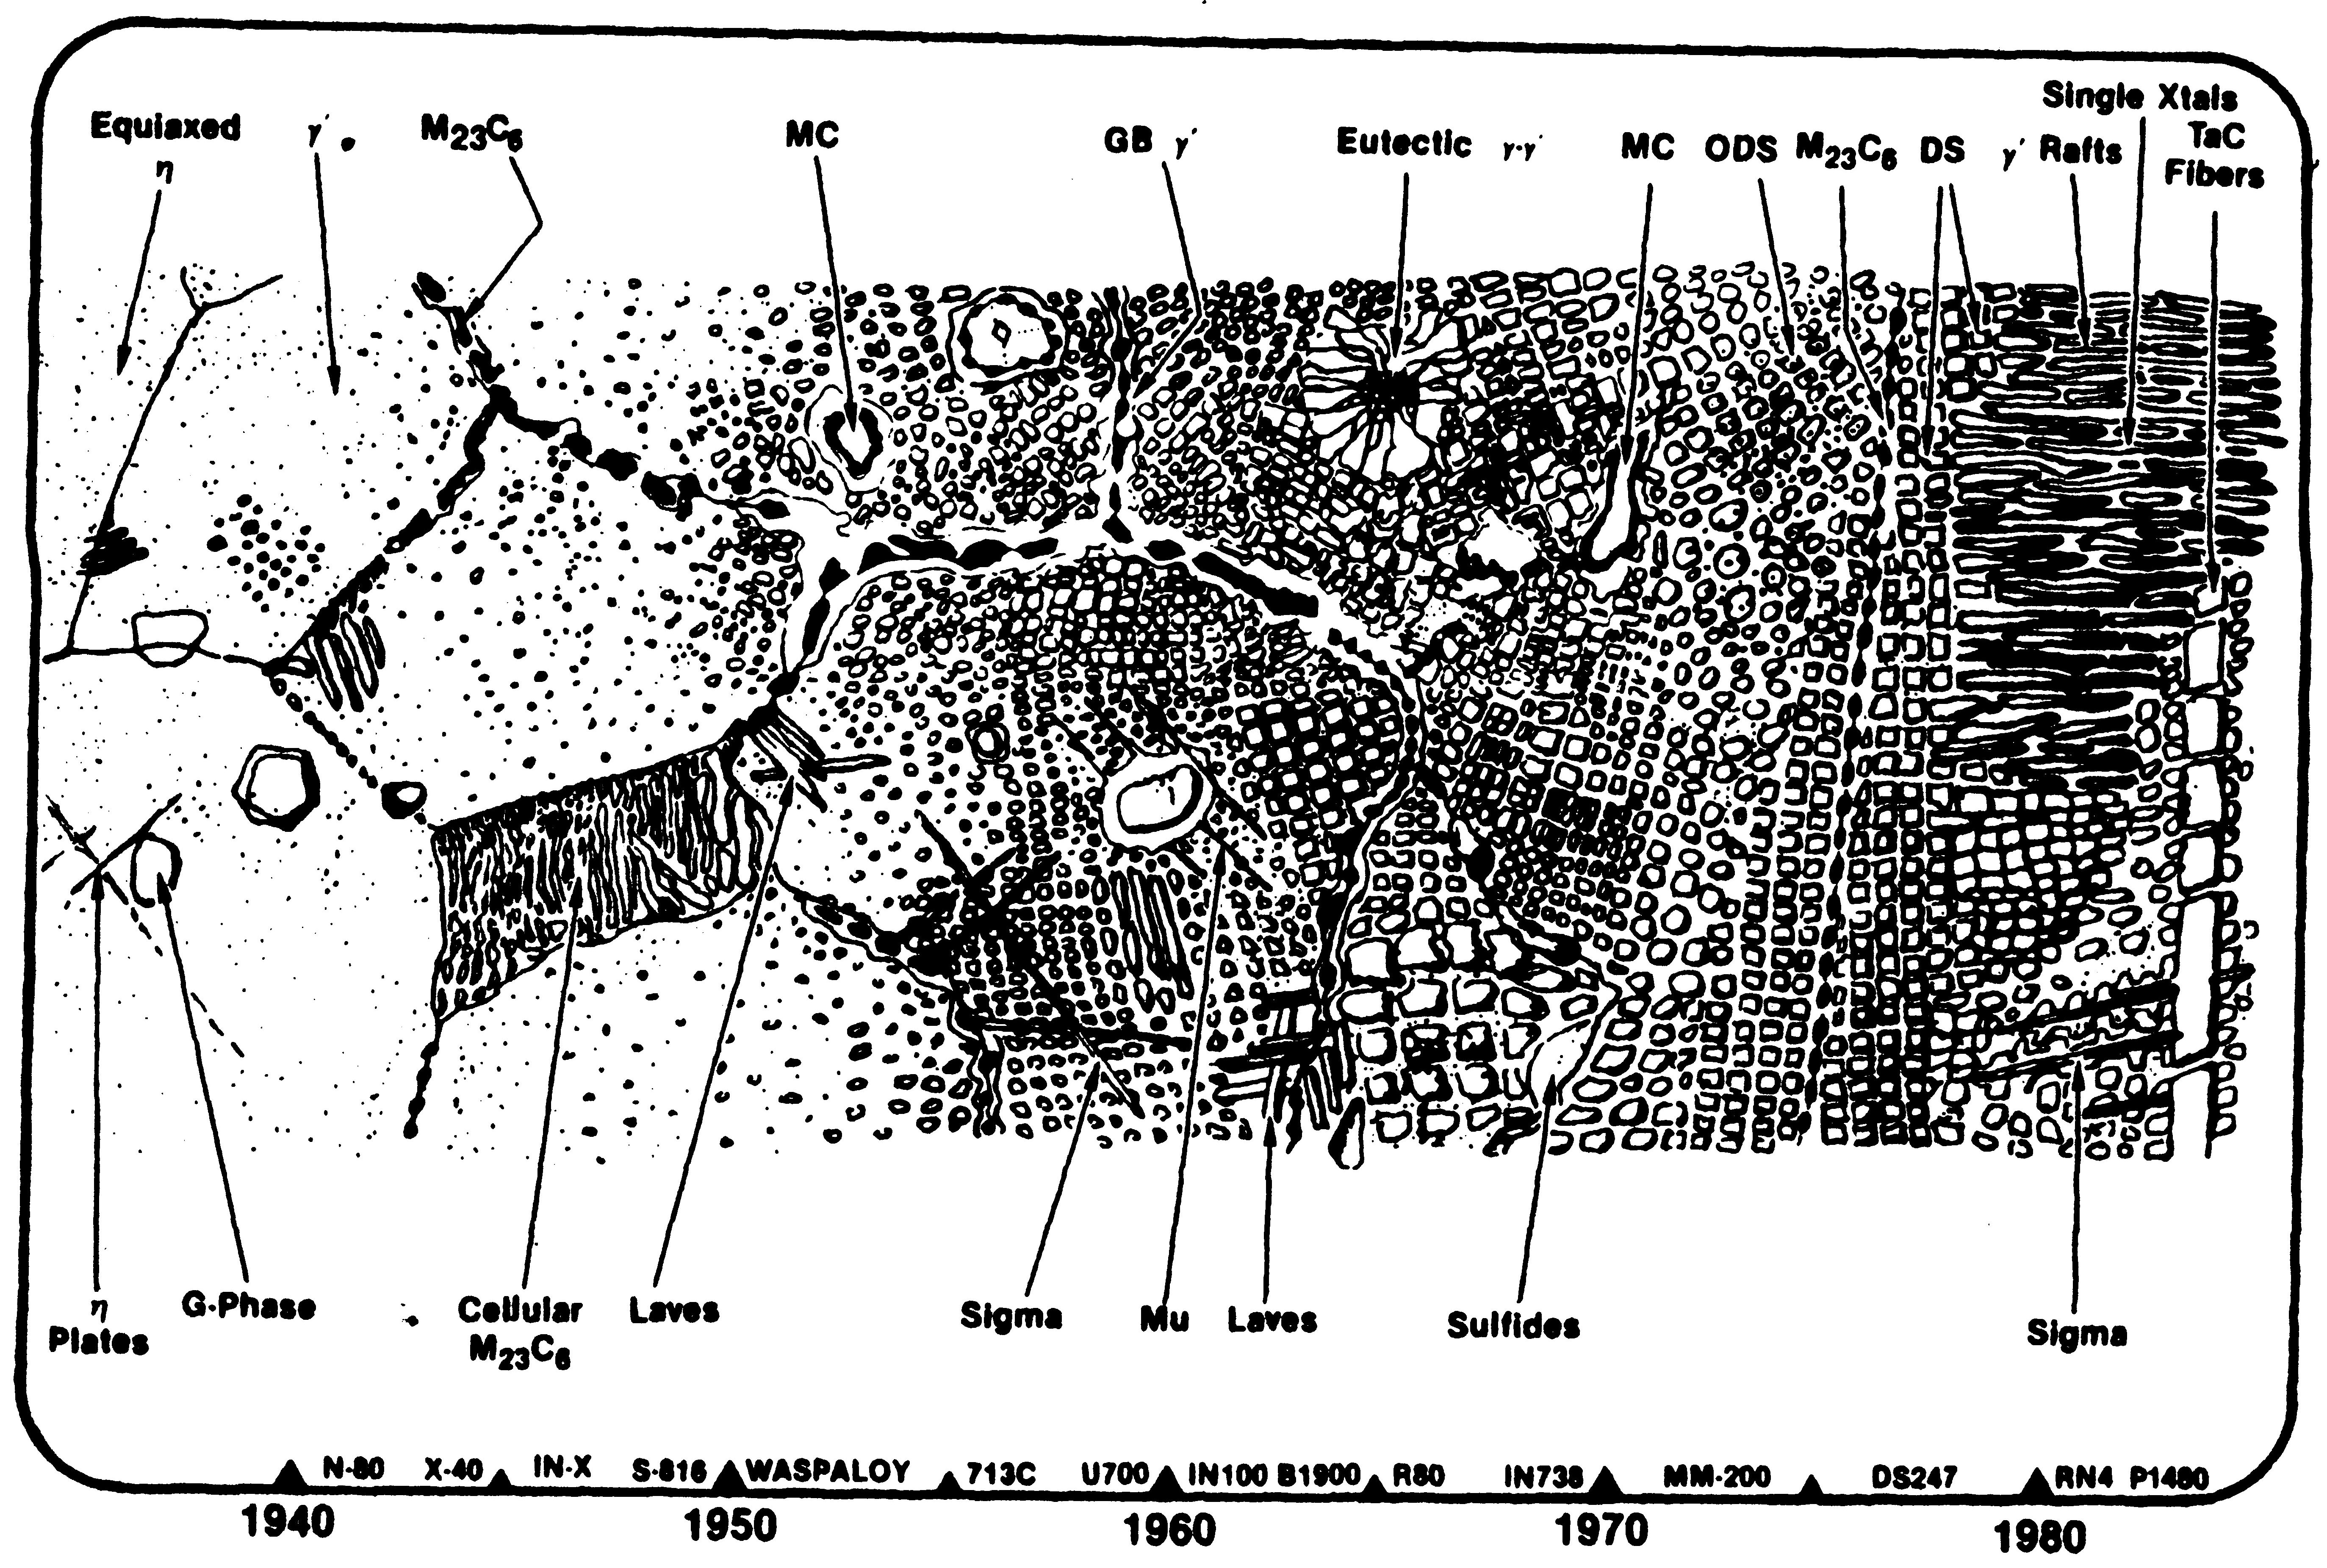
\includegraphics[height=5.5in, angle=90.6]{SuperalloyEvolution}
\caption{Evolution of blade material.  Panorama of the development of nickel superalloy microstructure showing both useful and deleterious phases \cite{sims87}.}
\label{fig:evolution}
\end{center}
\end{figure}
%
The superalloy started out with a multi-grained face-centred cubic (FCC) nickel-chromium austenite matrix, with carbides serving as the strengthening phase.  This choice of having an FCC matrix is rather fortuitous, as it is now known to be the atomic configuration that can best maintain strength to high homologous temperatures.  Aluminium was then found to effectively improve high temperature oxidation resistance, due to the transition of oxide structure from chromia to alumina.  Moreover, unbeknownst to the metallurgists, their additions of aluminium also created a small volume fraction of coherent Ni$_3$Al $\gamma'$ precipitates, the sole strengthening phase employed in the most advanced single-crystal nickel-base superalloys today. 

With the advent of electron microscopy a decade later, metallurgists were then able to identify carbides and $\gamma'$, and quantify their effects on the high temperature mechanical behaviour alloys.  This led to alloys being designed with increasing volume fractions of both phases.  Refractory elements were then found to impart strength to both the solid-solution and the precipitates.  Molybdenum was added, followed by tantalum and tungsten.  This compromised microstructural stability, and precipitated the formation of embrittling TCP phases.  These TCP phases serve as crack nucleation sites, inducing creep cavitation ~\cite{reed99} and causing premature creep failure at high temperatures ~\cite{yeh04}.  As these phases consist mostly of refractory elements, surrounding regions get depleted of their strengthening elements, and this exacerbates localized premature failure.  The threshold for solid-solution strengthening had been reached. 

Directional solidification manufacture was then introduced, allowing for crystal alignment and orientation.  Single crystal superalloys were made possible with the application of grain selectors.  This made carbides obsolete, as they were no longer necessary as grain boundary strengtheners.  This widened the heat treatment window and allowed for a more complete heat-treatment. 

In 1986, rhenium was discovered to effectively improve the high temperature mechanical properties of superalloys via solid-solution strengthening of the matrix.  Its low diffusivity in nickel at high temperatures was also found to interfere with diffusional creep mechanisms that occur at high temperatures.  Regrettably, its addition induced microstructural instability and inhomogeneity; 2 at.\% resulted in sufficient TCP precipitation to cause premature creep rupture.  The alloying ceiling had been reached again. 

Ruthenium was subsequently found to reduce this propensity for TCP formation by allowing superalloys to tolerate a higher rhenium content.  The crystal lattice has to undergo further distortion to accommodate these large refractory atoms, resulting in a more negative lattice misfit.  These superalloys suffer from premature creep failure at intermediate temperatures of 950\celsius, but the reasons for this have not been determined.

Although much of superalloy development has been empirical, the superalloy community is developing advanced modelling techniques to expedite the alloy development process.  Non-linear regression analyses and phase-diagram simulations are being used in the prediction of material properties and microstructure.  Finite element modelling is used in optimisation of solidification processes.  However, composition, microstructure and processing are very much inter-dependent.  Therefore, it is essential to couple models to incorporate all aspects of alloy design when designing a bespoke product with specific properties.

This is where the superalloys community stands currently.

\section{Microstructure and Deformation}

In order to understand the consequences of rafting at intermediate temperatures and intermediate stress, it is necessary to detail the superalloy microstructure and its deformation mechanisms during creep in this regime.

\subsection{Dislocations}

The $\gamma$ phase is a nickel-base solid-solution with a disordered fcc lattice.  The $\gamma'$ intermetallic phase is a Ni$_3$Al fcc superlattice with the L1$_2$ structure.  There is a coherent cube-cube orientation  relationship between $\gamma$ and $\gamma'$, and coherent $\gamma'$ precipitates form when lattice misfit is small.  These precipitates serve as barriers to dislocation motion, hardening the material ~\cite{copley67}. 

For dislocation motion to proceed, precipitate circumvention or cutting must occur.  In commercial blade superalloys, looping of dislocations around precipitates is made difficult by having a high volume fraction of small, discrete particles of $\gamma$' \cite{reed06, copley67}.  The resultant narrow matrix channels increase Orowan stress.  Dislocation climb is limited by the diffusion rate of the elements at and around the dislocation, and its rate increases with temperature.  During precipitate cutting, an $\frac{a}{2}\left<110\right>$ matrix dislocation moving through an ordered superlattice forms an anti-phase boundary (APB).  The high energy associated with these APBs inhibit dislocation motion through the ordered precipitate.  To minimise this formation energy, the $\frac{a}{2}\left<110\right>$ dislocations typically accomplish precipitate cutting by travelling in pairs or in groups.  The distance between a dislocation pair is dictated by the formation energy of the APB between the dislocations in the precipitate, 
their elastic repulsion energy, the temperature and magnitude of the applied stress.  When conditions are unfavourable for either mechanism to proceed, dislocation pile-up occurs at the matrix-precipitate interface, hardening the material.

%There is a driving force from elastic energy of dislocation strain fields for each superdislocation to dissociate into two $\frac{a}{2}\left<110\right>$ dislocations separated by an APB on the $\{111\}$ plane. 

As temperature rises up to 800\celsius, dislocations cross-slip so that the APB fault lies on the $\{001\}$ plane where it has a lower energy.  The dislocations become sessile, forming Kear-Wilsdorf locks ~\cite{reed06}.  These locks are the cause of the yield stress anomaly, where yield strength increases with temperature.  Above 800\celsius, $\gamma'$ softening occurs because the threshold stress for unlocking becomes lower.

MacKay and Ebert hypothesized that the misfit dislocations in the $\gamma$/$\gamma'$  interface are present to relieve the interfacial strains arising from the large negative mismatch~\cite{mackay83}.  These dislocations are similar to those observed in the initial stages of coherency loss of the $\gamma'$ precipitate in long-time aged superalloys, having three-dimensional octagonal networks of $\frac{a}{2}\left<110\right>$ edge dislocations.  Misfit dislocations relax the internal strain energy of a material due to large misfit, therefore decreasing the internal energy of the system. 

Harada and coworkers are of the opinion that dislocations form networks in the $\gamma$ channels that serve as a barrier to precipitate shear, and that these networks hinder the dislocations from entering the vertical $\gamma$ channels.  They hypothesize that superalloys with denser networks would be more resistant to high temperature creep ~\cite{harada06}.

As creep resistance is inversely related to the rate of dislocation motion, an effective means of hindering dislocation motion is precipitate volume fraction optimisation.  The optimal $\gamma'$ volume fraction would minimise the widths of the matrix channels between the precipitates whilst maintaining discrete precipitates.  Dislocations must bow more to enter the matrix channels, which requires higher stress.  Refractory element additions are beneficial as they lower diffusion coefficients and their larger diameters strengthen the solid-solution, providing resistance to dislocation motion.


\subsection{Lattice Misfit}

As discussed previously, it is generally desirable for alloys to contain significant quantities of refractory elements to improve creep performance.  Of these elements, only tungsten displays limited partitioning between the matrix and precipitates.  Molybdenum and rhenium partition preferentially to the matrix, whilst tantalum partitions to the precipitates ~\cite{reed04}.  In general, however, higher concentrations of refractory elements are typically in the matrix than in the precipitates.  The matrix thus has a larger coefficient of thermal expansion than the precipitates.  As a consequence, the lattice misfit is typically observed to become more negative upon heating.  This has a profound impact on the magnitude of the misfit seen in the alloy at elevated temperature depending upon the composition and hence also the room temperature misfit.

Lattice misfit quantifies the extent of coherency, with larger values signifying higher coherency strains, where the lattice parameter of the precipitate is substantially larger than that of the matrix, or vice-versa.  The lattice misfit is defined by \cite{nabarro96}:
%
\begin{equation}
\delta = \frac{2(a_{\gamma'} - a_\gamma)}{a_{\gamma'} + a_\gamma}
\label{eq:misfit}
\end{equation}
%
The mechanical properties of superalloys have been found to be heavily dependent on $\gamma$/$\gamma'$ interfacial coherency ~\cite{reed06}.  Dislocation movement is impeded by a high lattice misfit due to an increase in elastic strain in the slip plane.  For alloys with positive misfits at room temperature the misfits decrease in magnitude upon heating and may become negative.  In contrast, for an alloy with a negative misfit under ambient conditions, the magnitude of the misfit will typically increase monotonically upon heating. 

The fantastic creep performance of negatively-misfitting superalloys at 1100\celsius, a temperature very close to their homologous temperatures, is partly due to the rafts that form.  When superalloys of negative misfit raft, each raft is a large thin plate.  Dislocations are for the large part unable to travel further when they hit a raft of $\gamma$'.  When superalloys with a positive misfit raft, they form rods. Horizontal $\gamma$ channels weld together due to the load symmetry, and the two orientations of vertical channels remain unrafted and open.  At high temperature, when a dislocation travels through the ductile $\gamma$ solid-solution and impinges upon a rod, it is able to bow around the intermetallic rod quite easily.  This mechanism is conducive for creep.  Negative misfitting alloys thus demonstrate superior high temperature tensile properties.

With high misfit values, the interfacial energy increases, leading to a more rapid loss of coherency and an increase in the rate of precipitate coarsening.  With the discovery that ruthenium addition allows for increased refractory solubility, refractory element contents have increased, and misfit values have risen accordingly.  It is clear that these higher misfits will not allow coherency to be maintained at the precipitate-matrix interface.  Loss of coherency between the matrix and the precipitate, either by thermal relaxation or through the accumulation of dislocation debris following mechanical deformation, may lead to a reduction in the mechanical properties of the alloy.



\subsection{Creep}

Creep is a time-dependent mechanism of plastic deformation which occurs at stresses well below the stress required to cause extensive dislocation glide and can involve many different mechanisms including dislocation climb, grain boundary sliding and vacancy diffusion ~\cite{nabarro96}.  Reed states that Ni-based single crystal superalloys undergo three stages of creep deformation: primary, secondary and tertiary.  He identifies three regimes of creep: primary, tertiary and rafting \cite{reed99}. 

In this work, comments are restricted to the intermediate temperature/intermediate stress tertiary creep regime, with temperature between 850--1000\celsius, and stress between 300--500  \mega\pascal.  In this regime, the three stages of creep are not distinct; instead, there is minimal primary creep, and creep appears to increase logarithmically with time, as the strain-rate of creep is proportional to the accumulated macroscopic creep strain.

The relevant regime of creep plasticity for the intermediate stress/intermediate temperature creep condition of single crystal nickel-base superalloys is power law creep.  It essentially describes deformation produced by the glide of dislocations in the $\gamma$ phase.  This deformation is limited by dislocation climb around coherent $\gamma'$, which effectively serve as obstacles to prevent plastic flow.  Thermally activated diffusion allow dislocations to climb out of the slip plane, over $\gamma'$ precipitates, and continue to glide along another.  The creep rate is determined by dislocation density and the rate of dislocation movement, and is described by the Orowan equation \cite{nabarro95}:
%
\begin{equation}
\dot{\gamma}  = \rho  b  v  
\end{equation}
%
During high temperature creep, precipitate cutting is difficult due to the lower stress conditions experienced, and this results in dislocations being trapped within the $\gamma$ matrix channels.  Dislocation climb around the $\gamma'$ precipitates becomes the dominant mechanism (Figure \ref{fig:LDSX8disloc}).  Under intermediate temperature/intermediate stress creep conditions, some precipitate cutting occurs, but precipitate circumvention is dominant.  Under low temperature/high stress creep, the stress is experienced by the alloy is high enough to allow precipitate cutting as the principal mechanism for dislocation motion (Figure \ref{fig:LDSX1faults}).
%
\vspace{1cm}
\begin{figure}[H]
\begin{center}
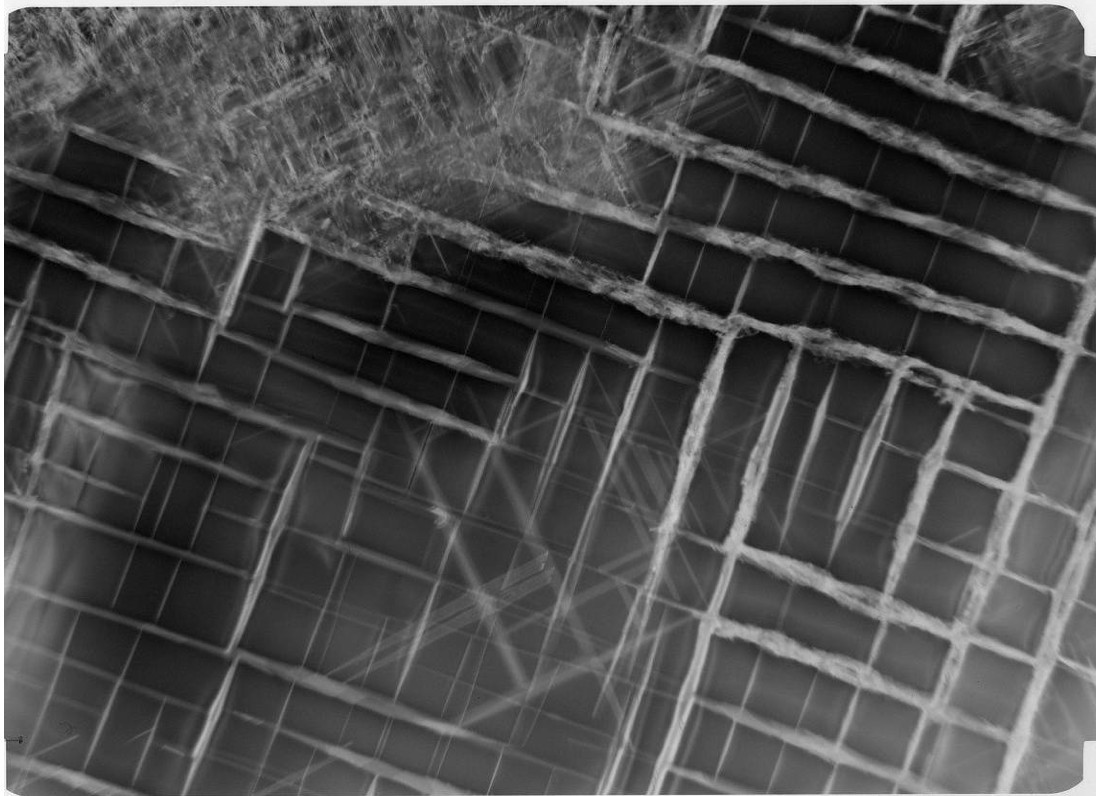
\includegraphics{LDSX8disloc}
\caption{Dislocations located mostly in the $\gamma$ channels of LDSX--8 after heat treatment; very few dislocations have entered the $\gamma'$ precipitates.}\label{fig:LDSX8disloc}
\end{center}
\end{figure}
%

\begin{figure}[H]
\begin{center}
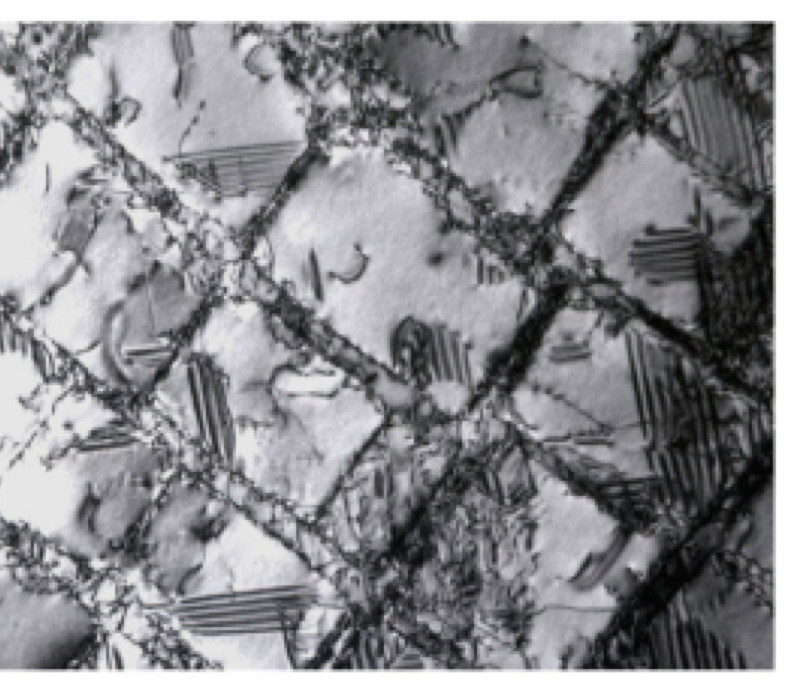
\includegraphics[width=8cm]{LDSX1faults}
\caption{Stacking faults in $\gamma'$ precipitates formed due to dislocation cutting in LDSX--1 after low temperature creep at 750\celsius/800 \mega\pascal.}\label{fig:LDSX1faults}
\end{center}
\end{figure}
%

\subsection{Rafting}\label{Rafting}
When a negatively-misfitting alloy is subject to tensile stress at elevated temperatures of above 900\celsius, dislocations form and accumulate in the horizontal channels, relieving the misfit stresses and allowing for the relaxation of coherency stresses on the horizontal $\gamma$/$\gamma'$ interfaces (Figure \ref{fig:CoherencyStress}).  This coincides with the cuboidal as-aged $\gamma'$ precipitates coalescing into rafts normal to the tensile loading axis.  This process is known as rafting.  When extensive rafting occurs, the encapsulating $\gamma$ matrix will no longer remain interconnected (Figure \ref{fig:LDSX6rafts}). 
%
\begin{figure}[H]
\begin{center}
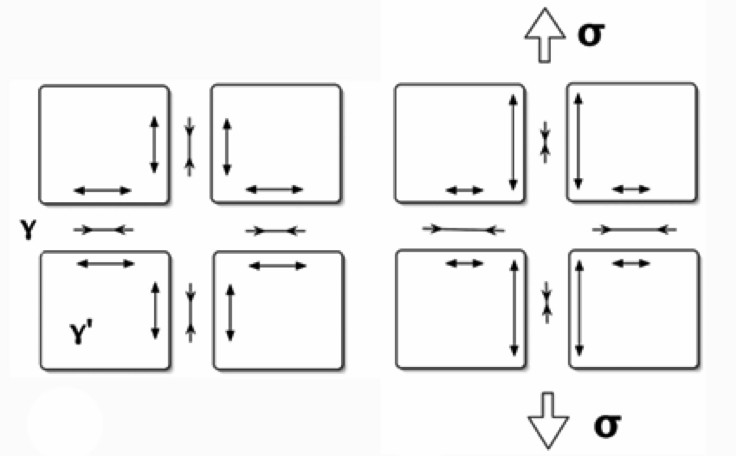
\includegraphics[width=10cm]{CoherencyStress}
\caption{Schematic of coherency stresses arising from an applied tensile stress (adapted from \cite{reed06}).}
\label{fig:CoherencyStress}
\end{center}
\end{figure}
%
\begin{figure}[H]
\begin{center}
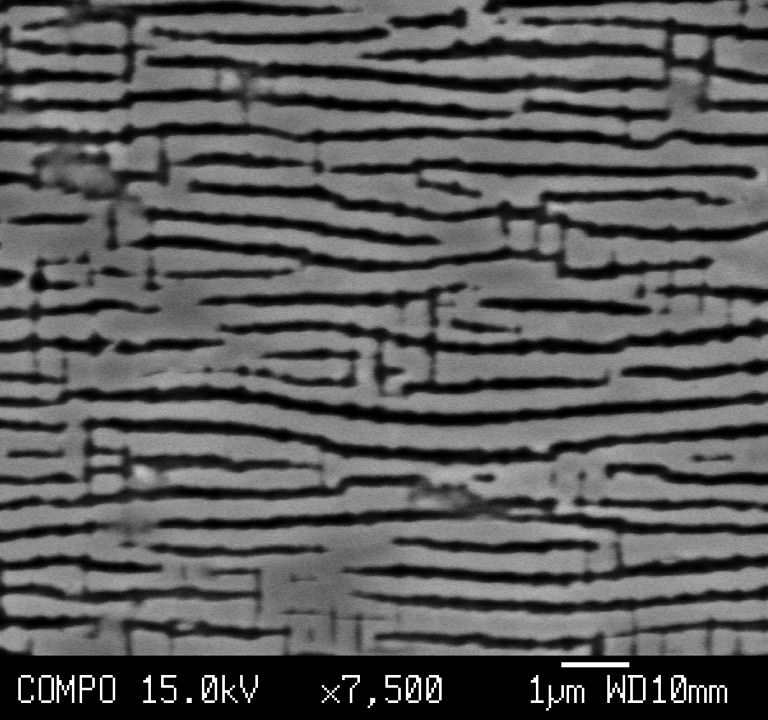
\includegraphics{LDSX6rafts}
\caption{Rafted microstructure of LDSX--6 interrupted after primary creep and subsequent thermal exposure for 500 hours at 950\celsius. }
\label{fig:LDSX6rafts}
\end{center}
\end{figure}
\vspace{-1cm}
%
In the early 1980s, rafting was believed to weaken the alloy's creep properties, due to the increase in inter-lamellar spacing.  Larger inter-lamellar spacing translates to larger $\gamma$ channels, which do not hinder dislocation motion.  This led to the development of alloys with lower lattice misfit, to obtain minimum coarsening rates with the intention of maximizing creep resistance.  MacKay and Ebert then reported that directional coarsening in single-crystal superalloys with large negative misfit increased creep life by 4 times in the $\left<100\right>$ orientation at 982\celsius\ \cite{mackay83}.  They found rafts were effective barriers to dislocation climb around $\gamma'$.

They observed that once rafts were formed during steady-state creep, the lamellae stabilise and do not undergo further rafting.  A limit had been reached where substantially higher amounts of total strain was required to induce further rafting.  From this, they hypothesised that rafting may be a strain-controlled and time-dependent phenomenon.

Factors influencing rafting kinetics are still a subject of controversy.  Reed et al. agree with MacKay's observation that the rafted structure is largely completed at the very early stages of deformation.  Since the rafts are established early, the dislocations, being unable to cut through them under the high temperature/low stress creep conditions, can only move via precipitate circumvention.  The plate-like morphology of these rafts makes circumvention very difficult.  This is probably why superalloys with rafted microstructure perform well during high temperature creep.

Although rafts are beneficial for high temperature creep, they have been found to be detrimental for creep at lower temperatures ~\cite{hobbs08}.  Blade alloys are subject to higher stresses at lower temperatures, this enables dislocations to cut through precipitates.  Since as heat-treated, uncoarsened cuboidal precipitates are finer than the ``rafts", dislocations have a larger energy barrier to surmount for precipitate cutting.  Also, they have a smaller average interparticle spacing, which impedes Orowan dislocation bowing, as the dislocation radius must be very large in order to have sufficient energy to force their way into the smaller $\gamma$ channels.


\section{Current Blade Superalloy Design Strategies}

At present, there are very few institutions conducting research to maximise the creep properties of single-crystal blade superalloys that can operate at temperatures at 1100\celsius\ and above.
The National Institute for Materials Science (NIMS) of Japan is one such institution.  Extensive research is being conducted at its High Temperature Materials Centre.  Since its inception, they have designed about 250 alloys and their derivatives by employing a largely empirical strategy.  Several of the cutting-edge single-crystal blade superalloys produced over the last decade have been designed at this centre.  A vast amount of material property data from the analysis and testing of these superalloys has been acquired.  These include tensile creep data at low (750\celsius), medium (950\celsius) and high (1000-1100\celsius) temperatures, propensity for TCP precipitation, lattice misfit at various temperatures, estimates of oxidation character, and phase partitioning behaviour of elements added to alloys.  This data has been analysed statistically using linear regression and organised in a database/program called the Alloy Design Program (ADP) ~\cite{harada88}.  The effect of changing a particular element’s content on any of the quantified properties can be determined through interpolation using the APD.  Alloys within the composition range quantified in the ADP can have their properties predicted with a reasonable degree of accuracy.  ADP has poorer property predictions for atypical alloys, such as superalloys with high rhenium contents of over 5at.\%.

%
\begin{table}[htdp]
\begin{center}
\begin{tabular}{lcc}
\hline\hline
Physical Property	&	\\
\hline
$\gamma$' atomic fraction at 900\celsius& \\
Yield stress (MPa) at 900\celsius\ &	\\ 
Creep rupture life (polycrystalline)(h) at 1000\celsius/ 118MPa &	\\
Density (gramme\usk\centi\rpcubic\metre) &	\\
Creep rupture life (single-crystal) 1040\celsius/137MPa &	\\
Lattice Misfit at room temperature 	&	\\
Tensile Elongation at 900\celsius	&	\\
\hline
\hline
\end{tabular}
\end{center}
\caption{Properties of superalloys that can be estimated by the Alloy Design Program ~\cite{harada88}.}
\end{table}


%Although much of superalloy development has been empirical, the superalloy community is developing advanced modelling techniques to expediate the alloy development process.  
%Non-linear regression analyses and phase diagram simulations are being used in the prediction of material properties and microstructure. 
%Finite element modelling is used in optimisation of solidification processes.  
%However, composition, microstructure and processing are very much interdependent.
% Therefore, it is essential to couple models to incorporate all aspects of alloy design when designing a bespoke product with specific properties.  
%This is where the superalloys community stands at currently.

\subsection{The Solubility Index} 

At NIMS, a simple indicator is used to gauge an alloy’s propensity to precipitate TCP phases.  This has been termed the Solubility Index (S.I.) ~\cite{harada88}. 

The $\gamma$ matrix is a nickel-based solid-solution; the $\gamma$' precipitate, Ni$_3$Al, has basis in nickel and aluminium.  All other elements are considered as additions to the Ni--Ni$_3$Al system.  This allows us to use Ni-Al-X ternary diagrams as a basis for element comparison during alloy design.  Most of the elements that can contribute substantially to high temperature creep properties have lower solubility in the intermetallic gamma’ than $\gamma$ at all temperatures.  The maximum solubility of a given element X in $\gamma'$ has thus been termed the element's Solubility Limit (S.L.).  As the $\gamma'$ phase field tends to expand with increasing temperature, when possible, S.L. is determined across a typical range of operating temperatures (900--1100\celsius), rather than merely at room temperature.  This prevents precipitation of tertiary phases that have been shown to instigate premature high temperature creep rupture.  

Ni-Al-X ternary diagrams for elements used in superalloys have been displayed in Figures \ref{fig:SLi}, \ref{fig:SLii} and \ref{fig:SLiii}: Ta ~\cite{willemin86}, W ~\cite{alekseeva93}, Ru ~\cite{sokolovskaya85}, Co ~\cite{kainuma96}, Cr ~\cite{oforka85} and Mo ~\cite{kubaschewski93}.  Ternary diagrams at 1100\celsius\ and 900\celsius\ were obtained when they were available.  Experiments have found that the microstructural stability is more critical at such temperatures because diffusion at lower temperatures is not significant enough to effect substantial microstructural change.

Ta forms an L1$_2$ Ni$_3$Ta, and stabilises $\gamma$'.  The $\gamma$' phase field widens with Ta content (Figure \ref{fig:SLi}).  W is substantially more soluble in $\gamma$, and has 5-8at.\% solubility in $\gamma$' at 1250\celsius\ (Figure \ref{fig:SLi}) ~\cite{hong89, udovskii91}.  Co does not form Co$_3$Al, but its complete miscibility with Ni is purported to aid in element dissolution in the alloy.  Co creates an extended $\gamma$' phase field, allowing for microstructurally stable alloys with up to 20at.\% Co content at 1100\celsius\ ~\cite{kainuma96}.  This minimises TCP precipitation.   Mo is a potent solid-solution strengthener, but cannot be added at more than 6at.\% as it has a very small phase field in Ni$_3$Al, even at 1100\celsius\ (Figure \ref{fig:SLi}).  Cr has a slightly larger Ni$_3$Al phase field than Mo, and can be added up to about 7-8at.\%. Although Ru shrinks the $\gamma$' phase field, it has a large $\beta$ phase-field for NiAl and RuAl ~\cite{trety93}.

The Solubility Index of an alloy is calculated using these ternary diagrams.  Take the fraction of every element’s concentration in the alloy over the its maximum possible concentration in the $\gamma$' phase as shown in the Ni-Al-X ternary; the Solubility Index would be the summation of all fractions.

	S.I. = C$_{element 1}$/S.L.$_{element 1}$ + C$_{element 2}$/S.L.$_{element 2}$ + … C$_{element x}$/S.L.$_{element x}$


where: 
\begin{itemize}
\item[] S.I. is the Solubility Index.
\item[] C$_{element}$ is the concentration of an element in the alloy. 
\item[] S.L. is the Solubility Limit of element X in the $\gamma$' phase field in the Ni-Al-X ternary at 1100\celsius.  
\end{itemize}  

In earlier generations of superalloys that do not contain ruthenium, it has been empirically determined that their maximum solubility indices are between 1.0 and 1.05.  In the third generation superalloys with Ru contents of about 3at.\%, their maximum solubility indices have been found to be slightly higher, about 1.05--1.1.  In the latest generation superalloys with Ru contents of 5at.\%, maximum solubility indices can be up to 1.15.  If an alloy’s solubility index is reached, it will precipitate TCP phases upon thermal exposure.  As mentioned earlier, TCP precipitation in such advanced $\gamma$/$\gamma$' superalloys has been shown to result in premature creep failure.



%
\begin{figure}[H]
\begin{center}
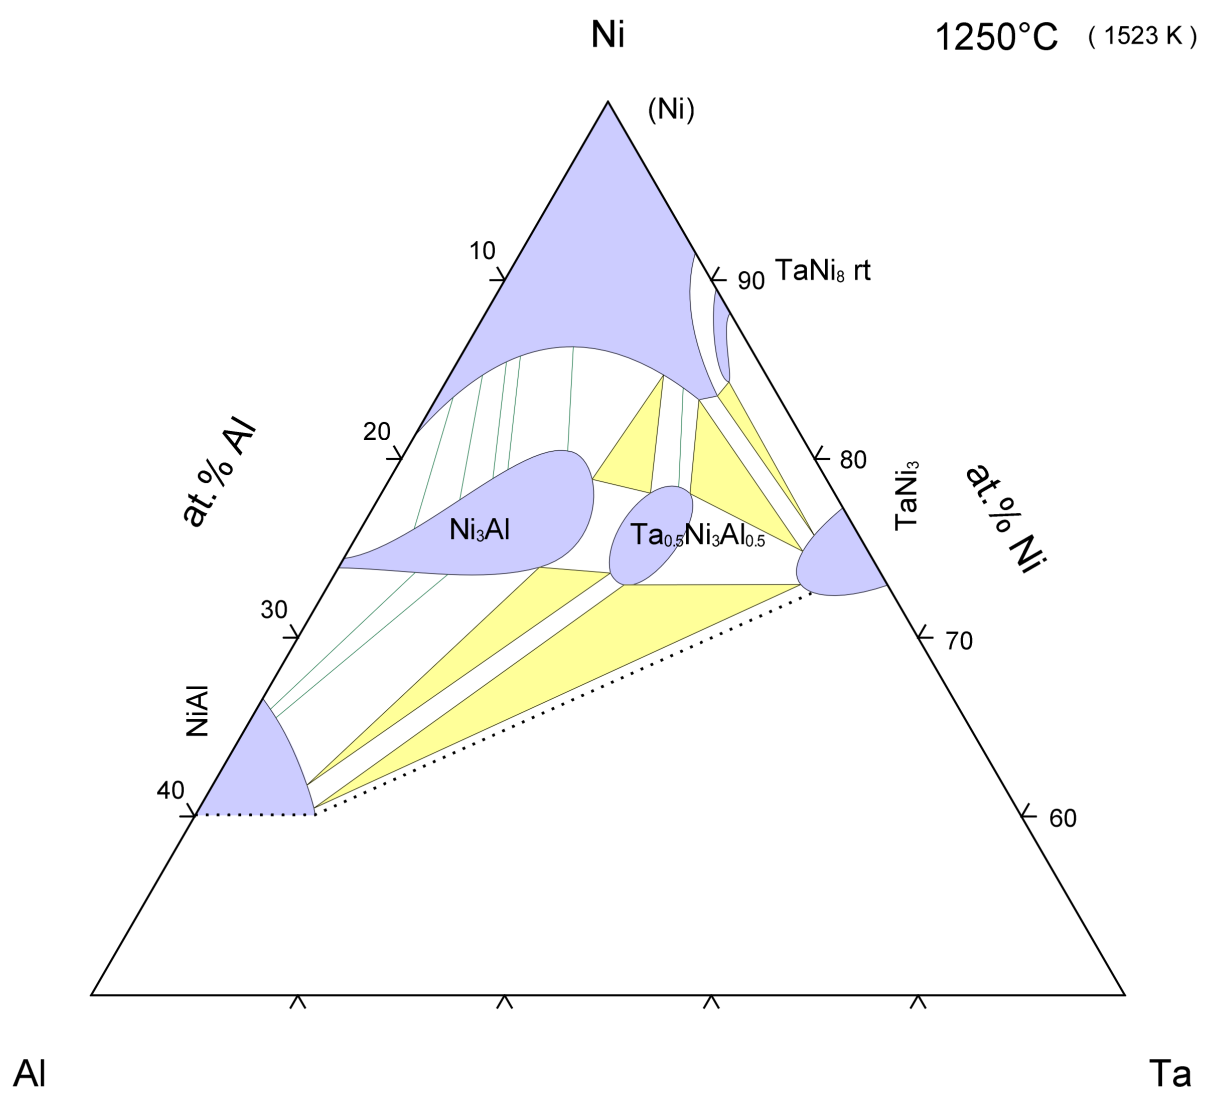
\includegraphics[width=12cm]{NiAlTa1250}
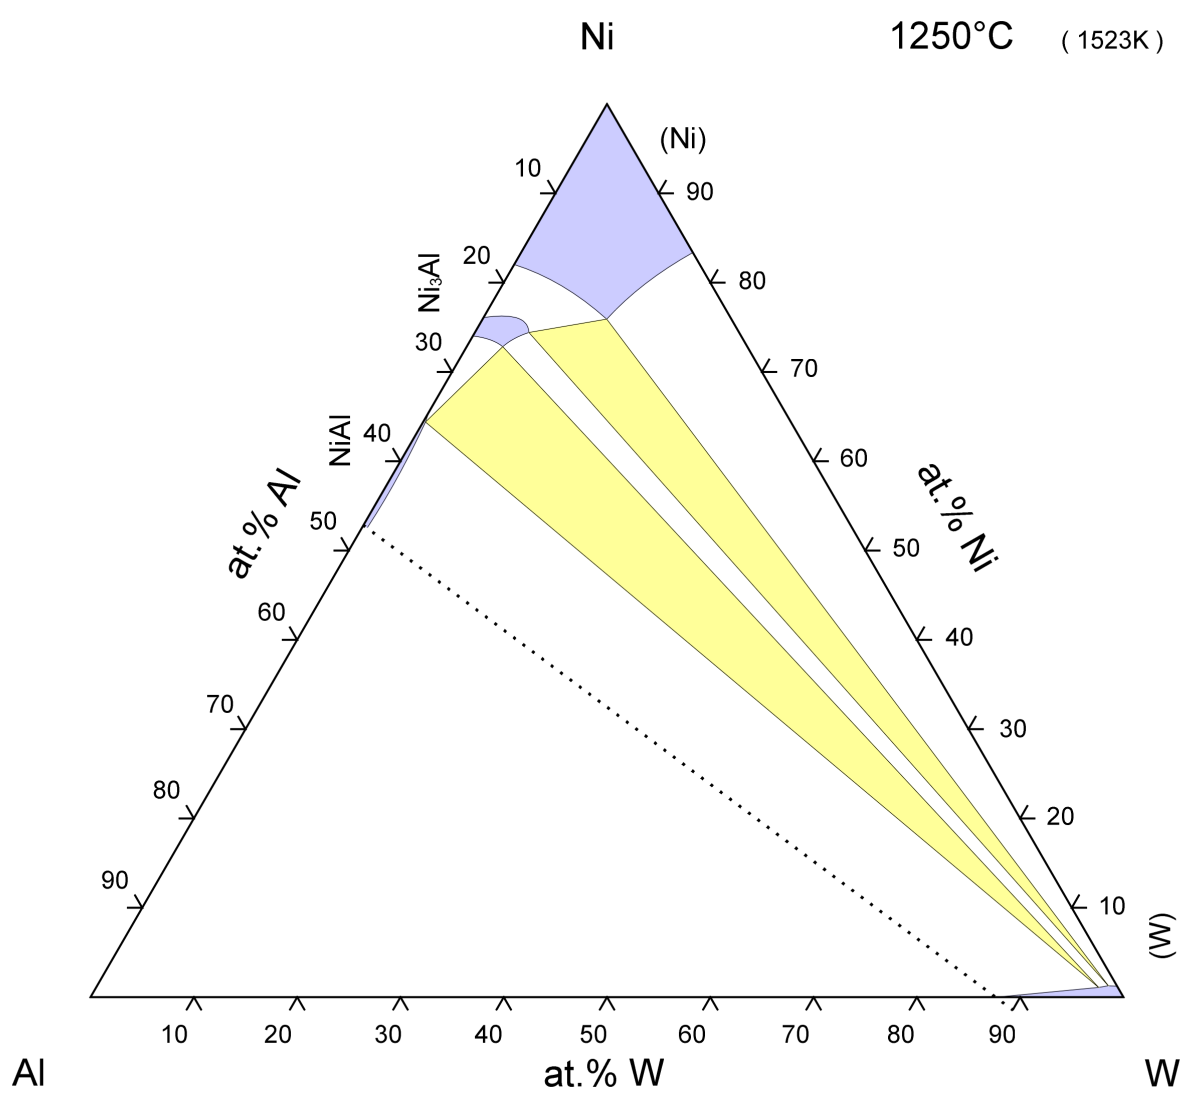
\includegraphics[width=12cm]{NiAlW1250}
\caption{Ni-Al-X ternary diagrams of major alloying elements in superalloys: Ta at 1250\celsius\ ~\cite{willemin86} and W at 1250\celsius\ ~\cite{alekseeva93}.}
\label{fig:SLi}
\end{center}
\end{figure}
%
\begin{figure}[H]
\begin{center}
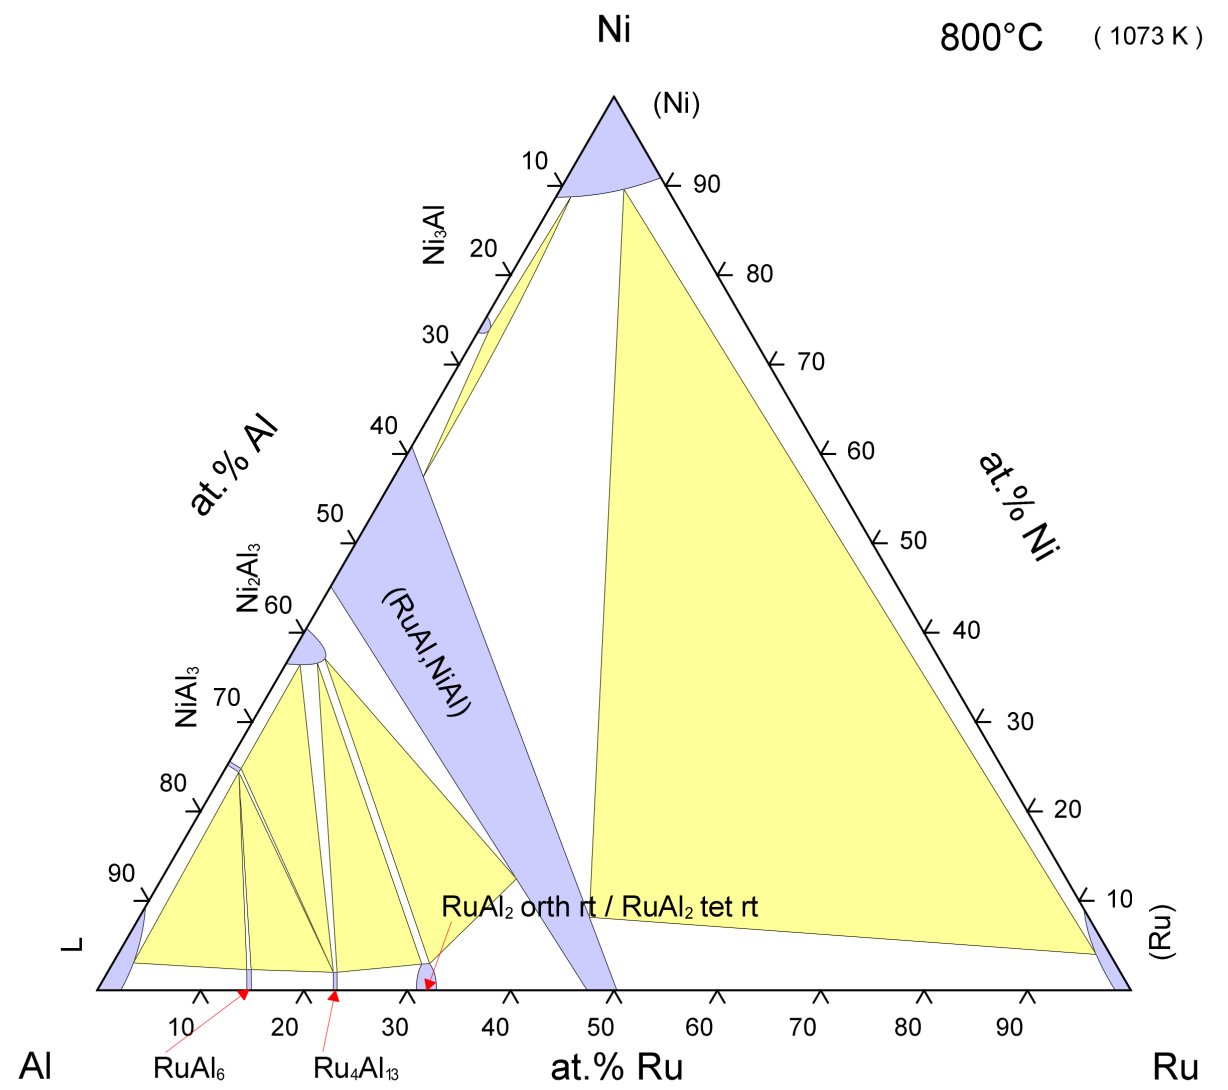
\includegraphics[width=12cm]{NiAlRu}
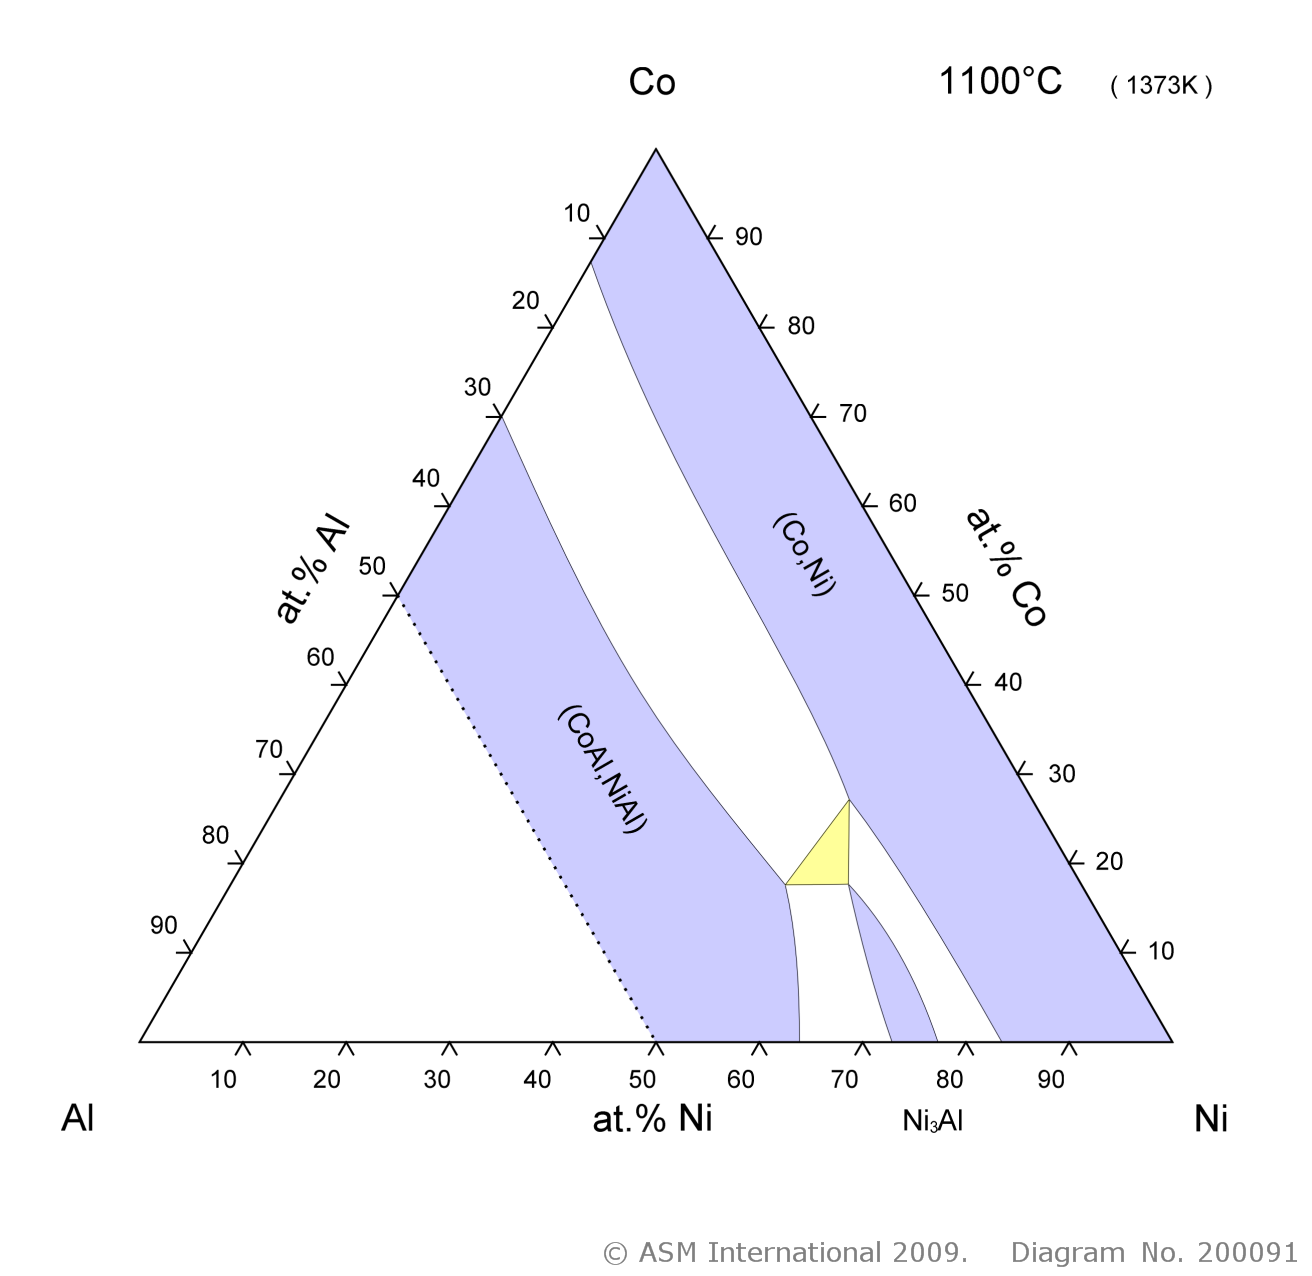
\includegraphics[width=12cm]{NiAlCo1100}
\caption{Ni-Al-X ternary diagrams of major alloying elements in superalloys: Ru at 800\celsius\ ~\cite{sokolovskaya85} and Co at 1100\celsius\ ~\cite{kainuma96}.}
\label{fig:SLii}
\end{center}
\end{figure}

%
\begin{figure}[H]
\begin{center}
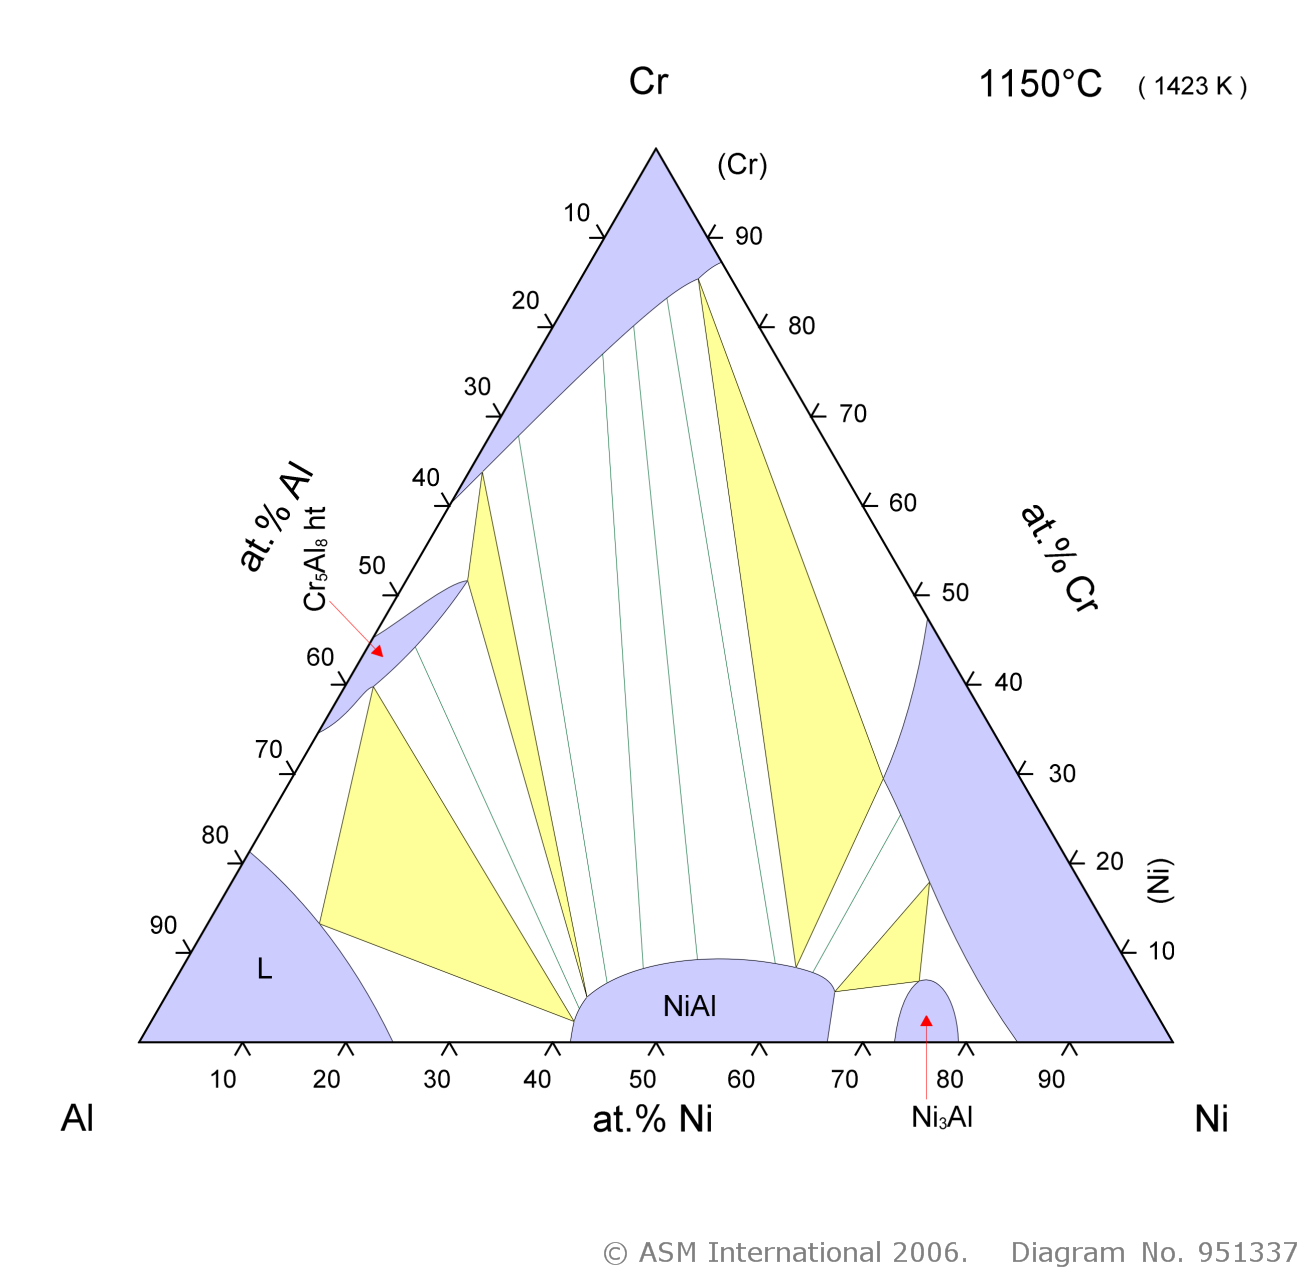
\includegraphics[width=11.5cm]{NiAlCr1150}
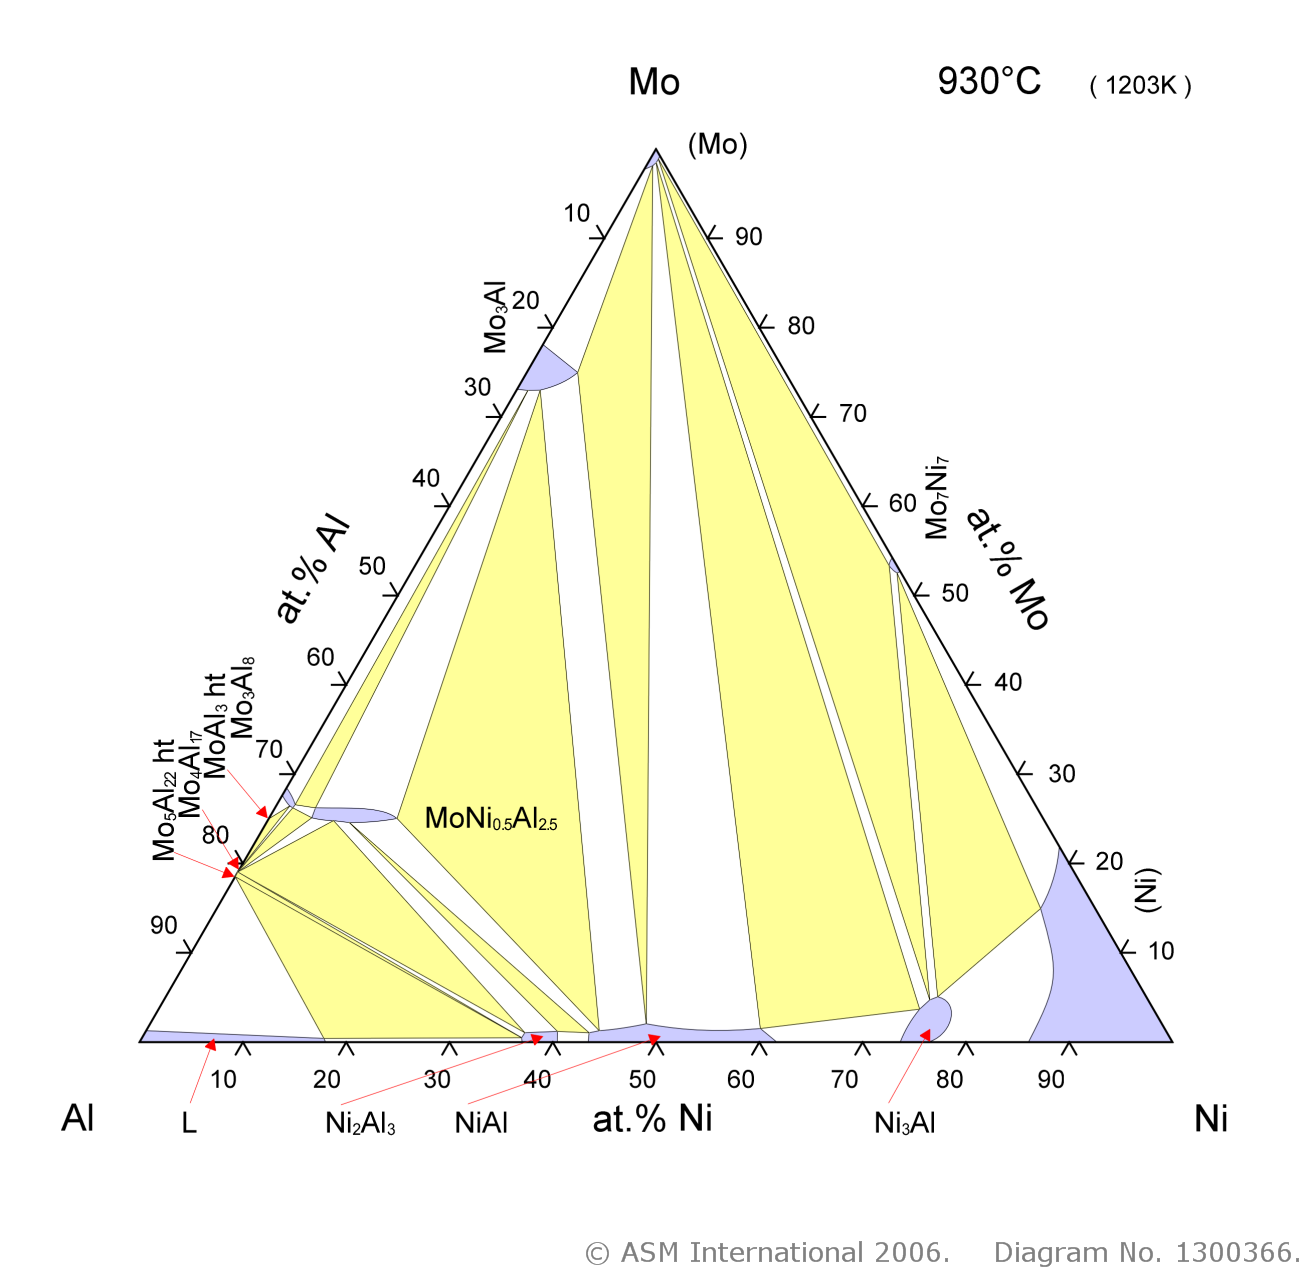
\includegraphics[width=11.5cm]{NiAlMo930}
\caption{Ni-Al-X ternary diagrams of major alloying elements in superalloys: Cr at 1150\celsius\ ~\cite{oforka85} and Mo at 1250\celsius\ ~\cite{kubaschewski93}.}
\label{fig:SLiii}
\end{center}
\end{figure}
%

It may seem counter-intuitive that the addition of Ru allows refractory element content to be increased in superalloys, as it does not increase the phase field of $\gamma$'.  Instead, it creates large $\gamma$ and $\beta$ phase fields.  The latter may, in alloys with very high refractory element content, help to preferentially stabilise $\gamma$' over $\gamma$; this may account for the suppression of TCP precipitate nucleation.

The solubility indices of superalloys are typically calculated only for 1100\celsius.  It was assumed that diffusion was most significant at this temperature and would thus escalate TCP nucleation and precipitation if they were to occur.  However, a good portion of $\gamma$' dissolves into the matrix, which possibly increases the solubility limit of the alloy.  Ideally, a superalloy should be designed with a solubility index that is less than its maximum at all temperatures up to the operating temperature.  If this is not feasible, one would need to pick a temperature at which diffusional processes have kicked in, but substantial $\gamma$' dissolution has not occurred.  This may be between 850 and 1050\celsius, and is dependent on the $\gamma$ dissolution temperature of the alloy.

\section{Manipulation of Oxidation Character in Superalloys}

Sufficient oxidation resistance is defined by the superalloy’s ability to form a thin (1-5 \micro\metre), adherent, oxygen-impermeable oxide layer upon exposure to high temperature.  An oxide scale consisting of a sole $\alpha$-alumina layer is the bench-mark of good oxidation resistance.  The superalloy must be able to regenerate the alumina layer if the oxide scale were to spall off due to thermal cycling or foreign object impact.  If this regeneration did not occur, runaway oxidation would result, and the component would see catastrophic failure.

If one wanted to improve the oxidation and corrosion characters of a superalloy, the approach would be rather simple.  The aluminium and chromium contents have to be increased, and the contents of elements that produce volatile or less-adherent oxides have to be reduced.  However, elements that improve oxidation character have to be present in contents that do not allow for their optimised contribution to high temperature strength.  The reduction of elements that produce non-ideal oxides would adversely affect the alloy’s high temperature creep properties.  This can be clearly seen in the work done in NIMS.  In the latest generation superalloys designed to possess the highest creep resistance at 1100\celsius, the elements that contribute positively to good oxidation character, Al and Cr, have had their contents lowered in order to accommodate other refractory elements known to improve high temperature strength.  These alloys, TMS-138, -162 and -173, although creep resistant, form thick, oxygen-permeable oxide scales that are spallation-prone. 
\clearpage
\section{Superalloy Design Strategy as Inspiration for Alloy Design Philosophy Employed in Alternative Materials Study}

There are many case studies on property optimisation in advanced superalloys.  The myriad of complications encountered in such studies  illustrates that many factors have to be considered in order to put together a sensible alloy design approach.  Grasping in the dark is an inadvisable approach, especially when dealing with a huge design space that has been somewhat explored, as in the case of alternative materials. 

An effective alloy design philosophy may be to maximise high temperature mechanical properties empirically in the first instance.  If the designed alloys show promising high temperature strength, sacrificing a portion of the alloying additions to increase the contents of elements that contribute positively to oxidation character can then be looked at. 

Using oxidation testing as the first stage of alloy design could be seen as a sensible approach.  It is a quick and cheap way of eliminating alloy systems prone to pesting.  The data acquired during exploration of potential systems is quite comprehensive.  Silicides with the most promising high temperature mechanical properties such as Nb and Mo silicides are prone to pesting.  Silicides of W and Ta may have good high temperature properties, but have very high densities, have poor oxidation resistance, and are prone to pesting.  Pesting is wide-spread, catastrophic, runaway oxidation of alloys at intermediate temperatues ~\cite{nesbitt93, shah92}.  Silicides that are not prone to pesting, such as Cr silicides, tend to have inferior mechanical properties.  However, it would be sensible to begin a systematic method of designing more advanced, multi-component alloys based on the information known.  Finding the extent that promising silicides can alloy with each other to produce feasible alloys with a better balance of properties would help paint a better picture of their synergistic potential.

To do this, we have adopted the empirical strategy for superalloy design described above to design our multi-component silicide alloys.  The concept of Solubility Index will be utilised to minimise the likelihood of unwanted phases forming.  This limited control over microstructure will control phase fraction somewhat, and enable a more direct comparison of results from high temperature mechanical testing.  The solubility of each element in all phases of the alloy will be determined through phase-diagram examination.  The upper limit of each element’s concentration would be its maximum solubility in the phase with lower element solubility.  The relationship between temperature and solubility will be mapped if there is data at various relevant temperatures.  If a large change in solubility is found, and no phase transitions occur, the lowest solubility found at temperatures above 900\celsius\ will be used as the limit.  Diffusion is limited at temperatures lower than 900\celsius, and will initially be regarded as an insignificant contributor to microstructural instability, especially since ternary phase-diagram information is limited or not available for many of the promising silicide systems we want to explore.	

In the case of multi-component additions, determination of the solubility limits for different cases would be useful.  Multi-component alloys that contain only elements that form perfectly miscible phases with each other will have a different solubility limit to multi-component alloys that also contain elements that form phases that are different to those of the base alloy.  Coupling modelling to experimental data has been initiated for established silicide alloys.  However, since the design space for (Cr,V)--(Cr,V)$_3$Si alloys is unexplored, modelling should not be done until the viability of this system is determined.


